\documentclass[draftcls,onecolumn]{IEEEtran}

%% INCLUDING THE PREAMBLE
%%%%%%%%%%%%%%%%%%%%%%%%%%%%%%%%%%%%%%%%%%%%%%%%%%%%%%%%%%%%%%%%%%%%%%%%%%%
%                                                                         %
%                                 PREAMBLE                                %
%                                                                         %
%%%%%%%%%%%%%%%%%%%%%%%%%%%%%%%%%%%%%%%%%%%%%%%%%%%%%%%%%%%%%%%%%%%%%%%%%%%

%% PACKAGES
\usepackage[margin=1in]{geometry}
\usepackage[]{lineno}
\linenumbers
\usepackage[usenames,dvipsnames]{xcolor}
\usepackage{listings,amsmath}
\usepackage{microtype,todonotes}
\usepackage{fancyvrb}
\VerbatimFootnotes

%% GRAPHICS RELATED
\usepackage{graphicx}
\usepackage[outdir=./tmp/]{epstopdf}
\graphicspath{{../images/}{./}{./tmp/}}
\DeclareGraphicsExtensions{.eps, .pdf, .jpeg, .png}

%% CPATION SETUP
\usepackage{float}
\usepackage{caption}
\usepackage{subcaption}
\captionsetup{belowskip=12pt,aboveskip=4pt}

%% HYPERLINKS
\usepackage[debug]{hyperref}

%% BIBLIOGRAPHY
\bibliographystyle{ieeetr}


%% EQUATIONS
%\numberwithin{equation}{section}

%% LISTINGS
\lstset{ %
    language=C++,
    basicstyle=\footnotesize\ttfamily,
    numbers=left,
    numberstyle=\tiny\color{gray},
    stepnumber=2,
    numbersep=5pt,
    backgroundcolor=\color{white},
    showspaces=false,
    showstringspaces=false,
    showtabs=false,
    frame=single,
    rulecolor=\color{black},
    tabsize=2,
    breaklines=true,
    breakatwhitespace=false,
    title=\lstname,
    keywordstyle=\color{blue},
    commentstyle=\color{OliveGreen},
    stringstyle=\color{orange}
}
\DeclareCaptionFont{white}{\color{white}}
\DeclareCaptionFormat{listing}{\colorbox[cmyk]{0.43, 0.35, 0.35, 0.01}{\parbox{\dimexpr\textwidth-2\fboxsep\relax}{#1#2#3}}}
\captionsetup[lstlisting]{format=listing,labelfont=white,textfont=white,singlelinecheck=false,margin=0pt,font={bf,footnotesize}}
\lstnewenvironment{code}[1][]%
{ \noindent\minipage{\linewidth}
	\lstset{#1}
}
{\endminipage}

%% USER COMMANDS
\usepackage{isotope}
\newcommand{\iso}{\isotope}
\newcommand{\figurewidth}{\textwidth}
\newcommand{\micron}{$\mu$m}


\usepackage{algorithm}
\usepackage{algorithmic}

%% SUBVERSION INFORMATION
\usepackage{svn-multi}
\svnidlong
{$LastChangedBy$}
{$LastChangedRevision$}
{$LastChangedDate$}
{$HeadURL$}

%%%%%%%%%%%%%%%%%%%%%%%%%%%%%%%%%%%%%%%%%%%%%%%%%%%%%%%%%%%%%%%%%%%%%%%%%%%
%                                                                         %
%                                Start of Document                        %
%                                                                         %
%%%%%%%%%%%%%%%%%%%%%%%%%%%%%%%%%%%%%%%%%%%%%%%%%%%%%%%%%%%%%%%%%%%%%%%%%%%
\begin{document}
\title{Layered Detectors}
\author{Matthew J. Urffer}
\date{\today}
\maketitle


% Tables of Contents, Figures, Tables
\listoftodos
\tableofcontents
\listoffigures
\listoftables
\lstlistoflistings
%%%%%%%%%%%%%%%%%%%%%%%%%%%%%%%%%%%%%%%%%%%%%%%%%%%%%%%%%%%%%%%%%%%%%%%%%%%
%                                                                         %
%                              Start of Content                           %
%                                                                         %
%%%%%%%%%%%%%%%%%%%%%%%%%%%%%%%%%%%%%%%%%%%%%%%%%%%%%%%%%%%%%%%%%%%%%%%%%%%

\section{Introduction}
It has been observed that GS20 has a signficantly lower count rate per mass \iso[6]{Li} than other detectors measured at the Department of Nuclear Engineering Radiation Charaterization Labratories Neutron Irridiator.
It has been proposed by A. Mabe that the decrease in the count rate per mass \iso[6]{Li} could be explained by self-sheilding in the GS20 glass in which the large absorbtion cross section of the GS20 causes a depression of the flux within the detector volume.
The depression of flux within the detector volume then creates few neturon interactions and counts, which results in a lower count rate per mass absorber.
In order to determine if self-sheilding is responsible for this reducation a series of MCNPX calcuations are proposed in which the mass of the aborber is increased, as well as measuring the neutron flux in each cell.

\section{Methods}
MCNPX was used to simulate the neutron interactions for various mass fractions of \iso[6]{Li} in GS20 glass.
The cylindrical \SI{2}{\mm} thick detector was divided into 10 equal slices, each \SI{0.2}{\mm} thick.
In each cell the total number of $\iso[6]{Li}\left(\text{n},\text{t}\right)\alpha$ interactions was tallied by the use of a flux tally multiplied by the cross section, as well as tally the neutron flux.
This allows for the flux and reaction rate to plotted as a profile through the glass.

In order to use a plausable material composition for differnet mass fractions of \iso[6]{Li} the mole fraction composition of GS20 was scaled by the relative amount of \iso[6]{Li}.
If we represent each the mole fraction of the material of a vector (i.e. every position in the vector corresponds to the mole fraction of a differnet isotope or element), then the mole fraction of a ficticous composition may be estimated by scaling the entire ratio to the desired mass fraction (normalizing by the existing mass fraction).
This process is outlined in \autoref{algo:Composition}.
\begin{algorithm}
  \caption[Molar Composition Calcualtion]{Calculation of Molar Composition of Fictious Lithated Glass Materials}
  \label{algo:Composition}
  \begin{algorithmic}
  \REQUIRE $x$, the desired mass fraction
  \REQUIRE $x_\text{GS20}$, the mass fraction of \iso[6]{Li} in true GS20
  \REQUIRE $\vec{n}$ be the mole fraction of true GS20
  \STATE $\vec{n}_x \leftarrow \frac{x}{x_\text{GS20}}\vec{n}$
  \STATE $n_{\iso[6]{Li}} \leftarrow n_{x,\iso[6]{Li}}$
  \STATE $\vec{n}_x \leftarrow \vec{n} - \vec{n}_x$
  \STATE $\vec{n}_{\iso[6]{Li}} \leftarrow n_{\iso[6]{Li}}$
  \RETURN $\lVert \vec{n}_x \rVert$
  \end{algorithmic}
\end{algorithm}
The intial composition of GS20 is shown in \autoref{tab:GS20Comp}.

A short python script, \autoref{lst:material}, was used to create the other compositions for simulation.
The actual amount of \iso[6]{Li} in the detector was using the \verb+PRINT 40+ card in the MCNPX simulation, and then searching the the output file for the mass fraction of \iso[6]{Li}. 
\begin{table}
  \centering
  \caption[GS20 Composition]{Comparison of GS20 Mass Fraction Compositions }
  \label{tab:GS20Comp}
  \begin{tabular}{c|c c c c c}
  \toprule
  & \ce{SiO2} & \ce{MgO} & \ce{Al2O3} & \ce{Li2O} \\
  \midrule
  Spowart (1976) & 57 & 4 & 18 & 4.0 & 17.1 \\
  AST & 56 & 4 & 18 & 4 & 18 \\
  \bottomrule
  \end{tabular}
\end{table}


\section{Results}

Thus, the each simulated flux has a surface contribution to it\footnote{assuming an isotropic impingnet neutron source, which after moderation is not unreasonable}, and is not a purecenter of material flux measurment.
\begin{figure}
	\includegraphics[width=\textwidth]{GS20SelfSheildFlux}
	\caption[Flux Profile through GS20]{Neutron flux profiles in GS20 glass for various mass fractions of \iso[6]{Li} in lithiated glass. Lower mass fractions have a much lower flux due to the absorborbition of neutrons in the material.}
	\label{fig:Flux}
\end{figure}
\begin{figure}
	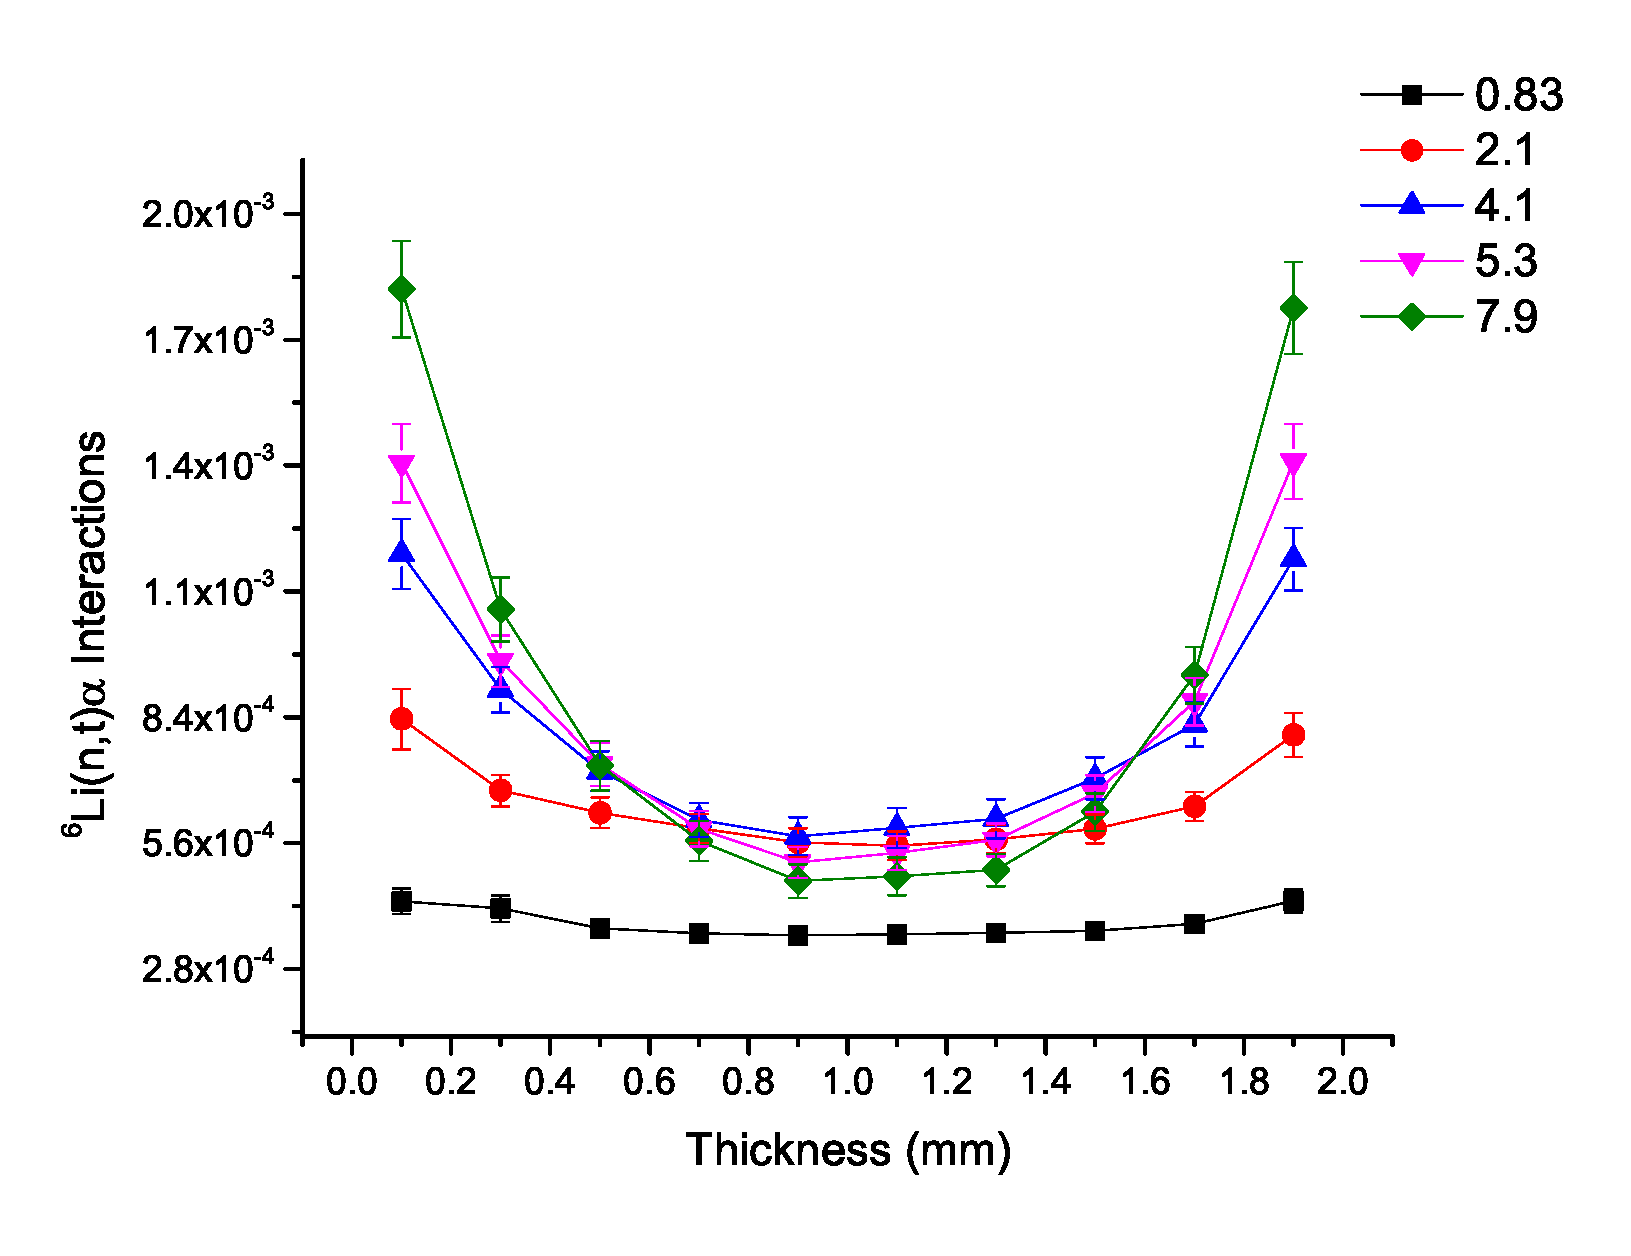
\includegraphics[width=\textwidth]{GS20SelfSheildRXNRate}
	\caption[Reaction Rate through GS20]{Reaction rate profile in GS20 for various mass fractions of \iso[6]{Li} in lithiated glass samples. It is observed that the highest interaction rates occur near the surface of the detector.}
	\label{fig:RxnRate}
\end{figure}
\begin{figure}
	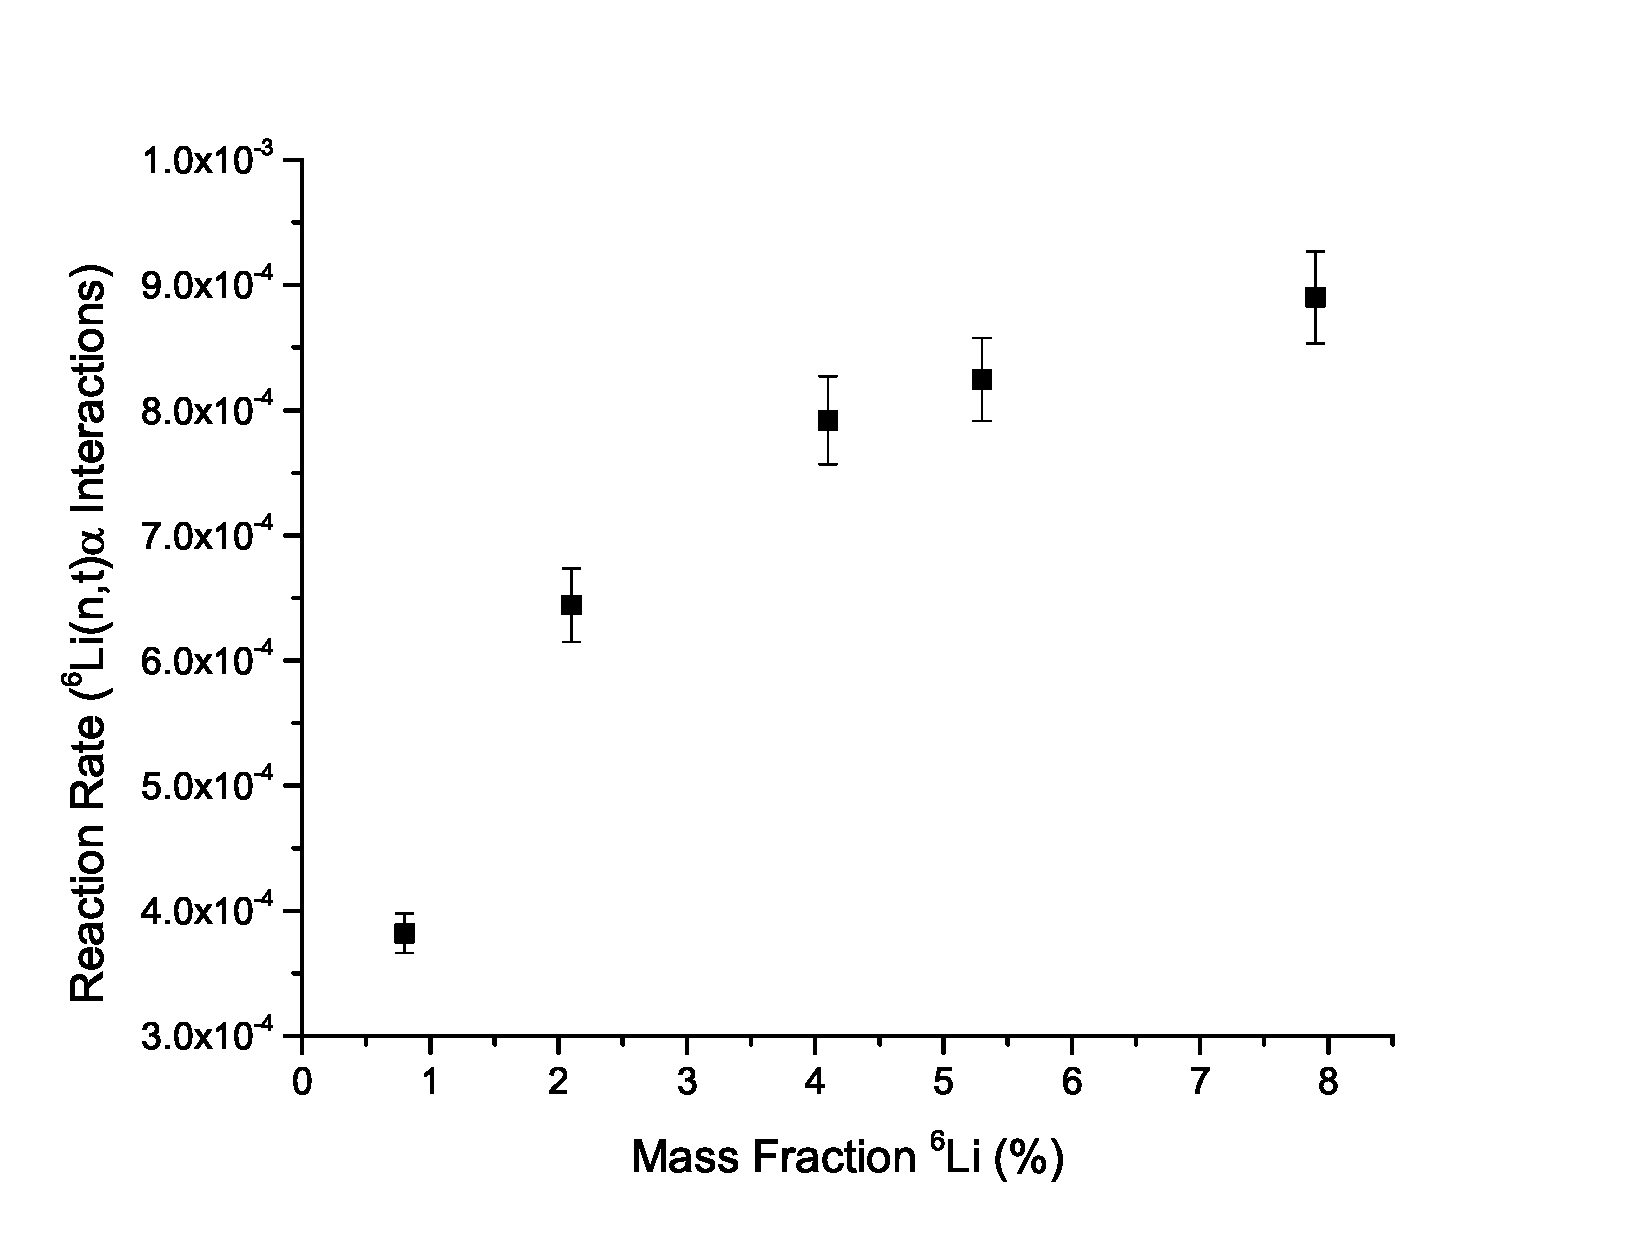
\includegraphics[width=\textwidth]{GS20SelfSheildTotal}
	\caption[Total Reaction Rate]{Total reaction rate in GS20 for various mass fractions of \iso[6]{Li} in lithiated glass samples}
	\label{fig:TotalRxn}
\end{figure}

\section{Appendix}
\label{sec:Appendix}
The various trials were completed by setting up a single MCNPX input deck (\autoref{lst:SCRIPT}) and then copying it and replacing the keywords to run with differnet materials, as shown in \autoref{lst:run}.
The material compositions were calculated with \autoref{lst:material}, whose output was copied directly into as the material compositions for \autoref{lst:SCRIPT}.
After all of the submitted jobs finished a python analysis script, \autoref{lst:analysis}, was used to extract the necessary tallies
using the \path{mctal.py} python class which reads in MCTAL files.
Finally, the data was plotted using OriginPro, with the plots saved in \path{Simulation/GS20SelfSheilding} of \path{MillerResearchPlots.obj}.
%%%%%%%%%%%%%%%%%%%%%%%%% LISTING CODE %%%%%%%%%%%%%%%%%%%%%%%%%%
\lstinputlisting[language=bash,caption=Run Script,label=lst:run]{SelfSheildSrc/run.sh}
\lstinputlisting[caption=MCNP Input Deck,label=lst:SCRIPT]{SelfSheildSrc/Miller_Config_GS20_SelfSheilding_Script.mcnp}
\lstinputlisting[caption=Python Material Composition Script,label=lst:material]{SelfSheildSrc/MoleFractionGS20.py}
\lstinputlisting[caption=Python Analysis Script,label=lst:analysis]{SelfSheildSrc/analysis.py}

The MCNPX output decks from which this analysis was based (and the corresponding python scripts) may be found in \path{/home/murffer/MCNP/GS20/SelfSheilding}.
This document is may be found in \LaTeX format at \url{\svnkw{HeadURL}}.  
The latest revision for this file is \svnrev, and was on \svndate, committed by \svnauthor.
\end{document}
